\begin{figure}[h!]
     \centering
    \captionsetup[sub]{font=small}
     \begin{subfigure}[b!]{0.25 \textwidth}
         \caption{}
         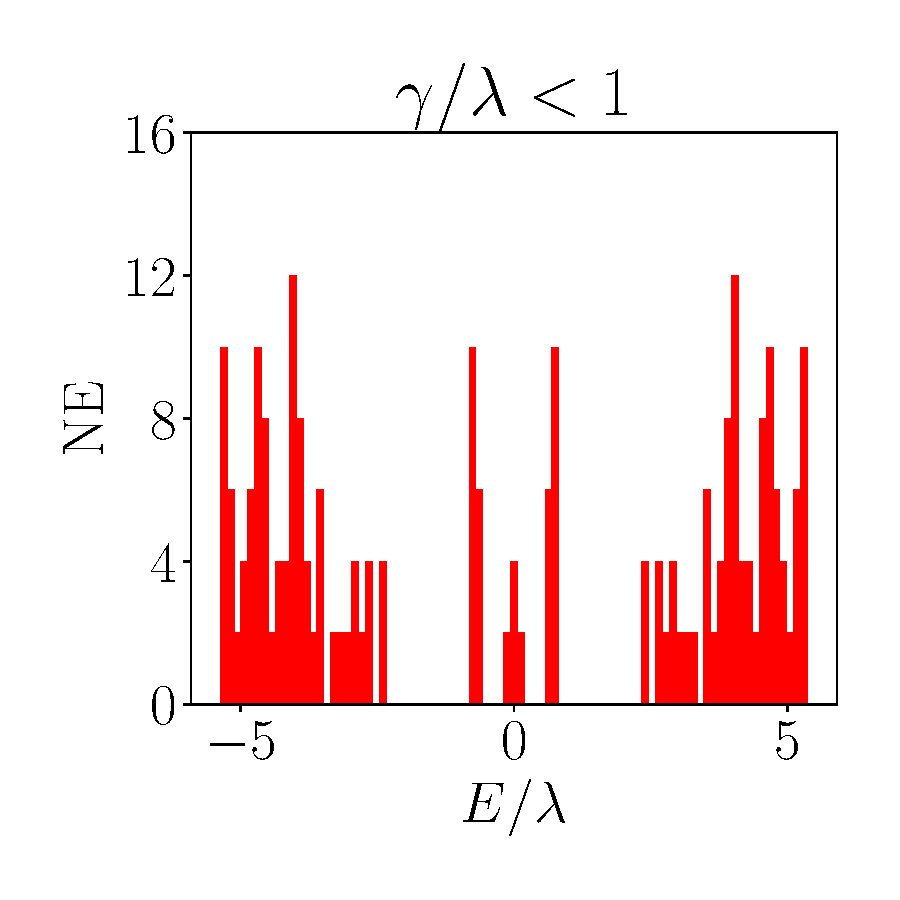
\includegraphics[width=\textwidth]{Imagenes/Resultados_Hoti_Fractal/bars_square1.pdf}
     \end{subfigure}\hspace*{-0.5em} 
     \begin{subfigure}[b!]{0.25 \textwidth}
         \caption{}
         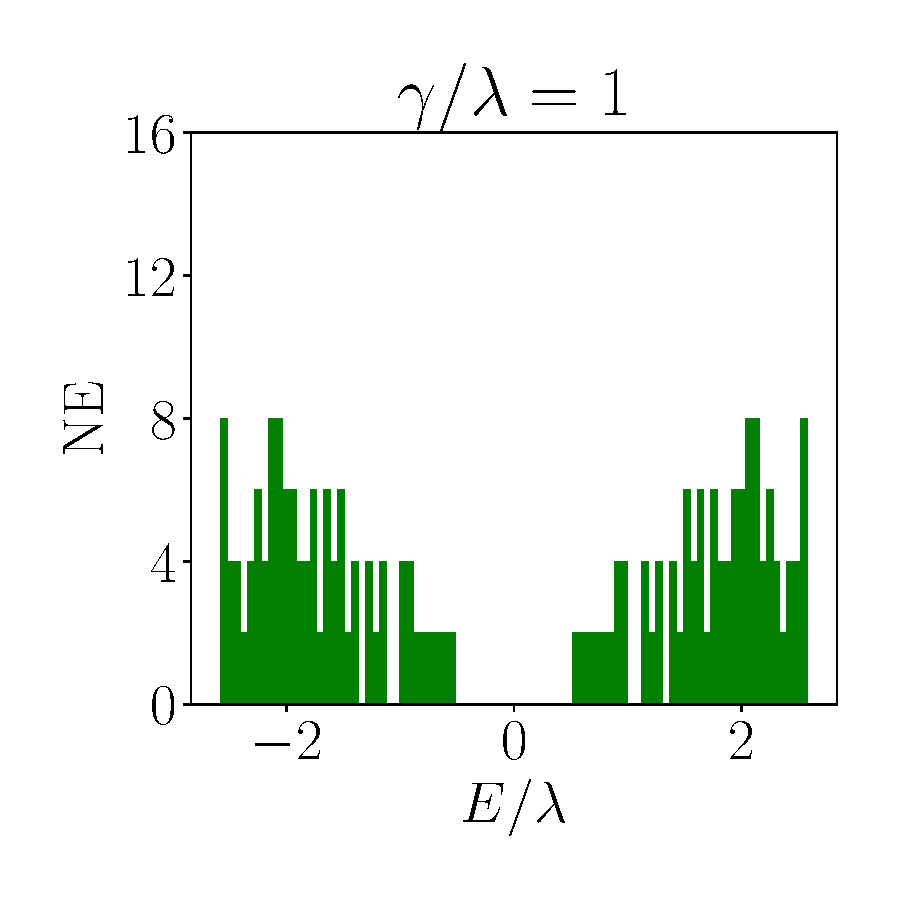
\includegraphics[width=\textwidth]{Imagenes/Resultados_Hoti_Fractal/bars_square2.pdf}
     \end{subfigure}\hspace*{-0.5em} 
     \begin{subfigure}[b!]{0.25 \textwidth}
         \caption{}
         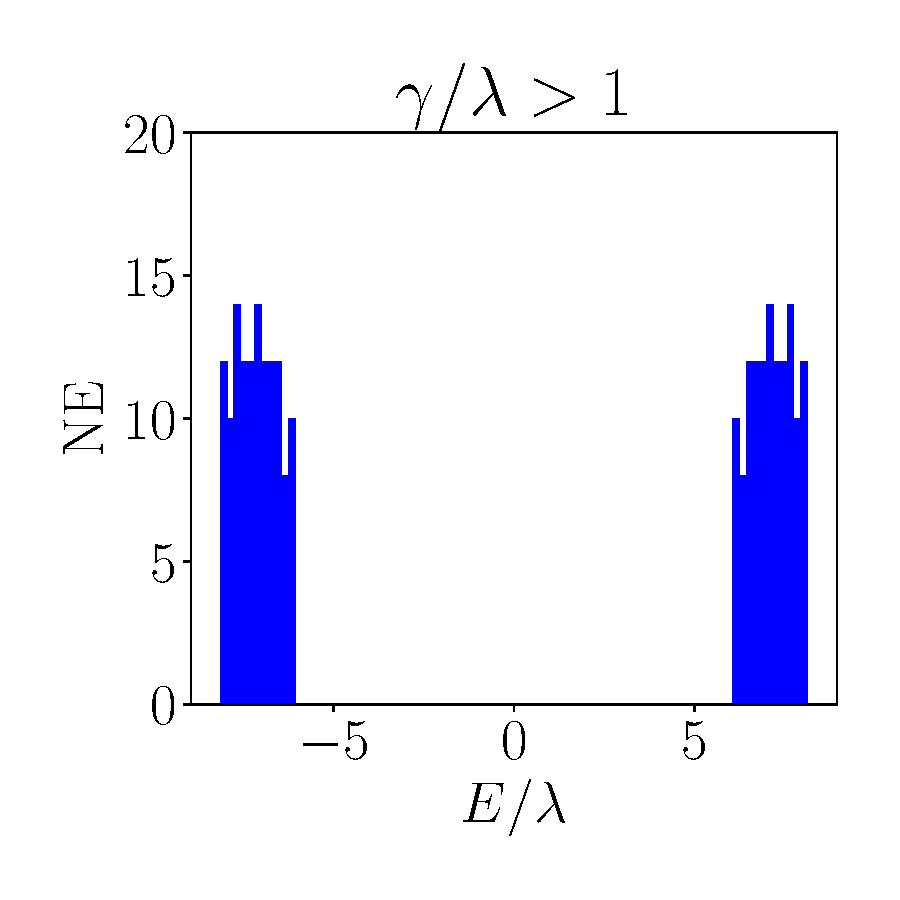
\includegraphics[width=\textwidth]{Imagenes/Resultados_Hoti_Fractal/bars_square3.pdf}
     \end{subfigure}\hspace*{-0.5em} 
     \begin{subfigure}[b!]{0.25 \textwidth}
        \caption{}
        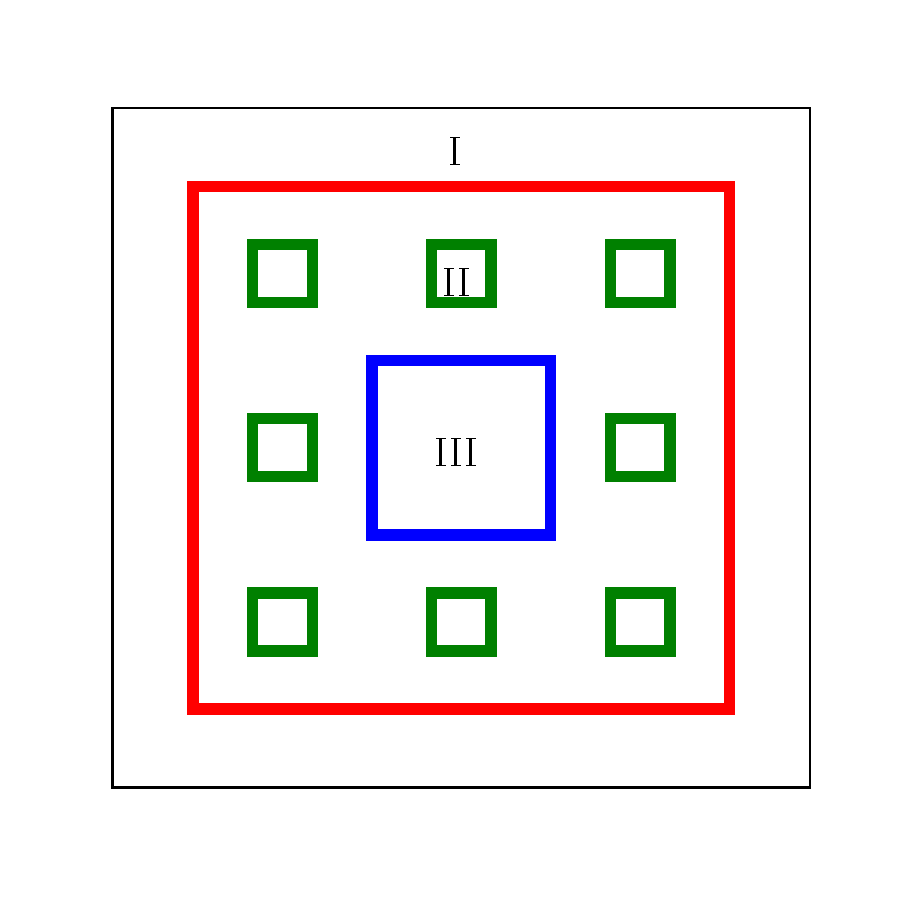
\includegraphics[width=\textwidth]{Imagenes/Models/sierpinski_carpet_color.pdf}
    \end{subfigure}\hspace*{-0.5em} \vspace*{-0.5em}
        \caption{Cantidad de estados por energía en un red con geometría Fractal (2da generación) para diferentes valores de los parámetros de salto, \textbf{(a)} $\gamma /\lambda = 1/2$, \textbf{
        (b)} $\gamma /\lambda = 1$, \textbf{(c)} $\gamma /\lambda = 2$. \textbf{(d)} Bordes de la red Fractal de Sierpinski de 2da generación.}
    \label{fig:Dos_fractal}
\end{figure}